\documentclass[aspectratio=169]{beamer}
\usetheme{Singapore}
\addtobeamertemplate{navigation symbols}{}{%
    \usebeamerfont{footline}%
    \usebeamercolor[fg]{footline}%
    \hspace{1em}%
    \raisebox{1.4pt}[0pt][0pt]{\insertframenumber/\inserttotalframenumber}
}
\setbeamercolor{footline}{fg=blue!50}
\setbeamerfont{footline}{series=\bfseries}

\usefonttheme[onlymath]{serif}

\usepackage{cmap}
\usepackage[english]{babel}
\usepackage[T1]{fontenc}
\usepackage[utf8]{inputenc}
\usepackage[kerning=true]{microtype}
\usepackage{lmodern}

\usepackage{amsmath}
\usepackage{amsfonts}
\usepackage{amssymb}
\usepackage{amsthm}

\usepackage{mathtools}
\usepackage{wrapfig}
\usepackage{enumitem}

\usepackage[
    backend=biber,
    style=numeric,
]{biblatex}
\usepackage{graphicx}

\graphicspath{{./images/}}

\addbibresource{../report/report.bib}
\renewcommand*{\bibfont}{\footnotesize}

\AtBeginSection[]
{
  \begin{frame}
    \frametitle{Plan}
    \tableofcontents[currentsection]
  \end{frame}
}


\theoremstyle{definition}
\newtheorem*{exemple}{Example}



\title{\textbf{Extending Layerwise Relevance Propagation using Semiring Annotations}}

\author{%
  \texorpdfstring{%
    \begin{columns}
      \column{.5\linewidth}
      \centering
      \textbf{Antoine Groudiev} \\ L3, ENS Ulm
      \column{.5\linewidth}
      \centering
      \textbf{Silviu Maniu} -- Supervisor \\ SLIDE Team, LIG
    \end{columns}
 }
 {Antoine Groudiev, Silviu Maniu}
}

\date{Tuesday, July 9th}

\begin{document}
\frame{\titlepage}

%\begin{frame}{Plan}
%    \tableofcontents
%\end{frame}

\section{Introduction}
\subsection{Problem statement}
\begin{frame}{Problem statement}

\end{frame}

\subsection{Layerwise Relevance Propagation}
\begin{frame}{Layerwise Relevance Propagation}
    \begin{figure}[H]
        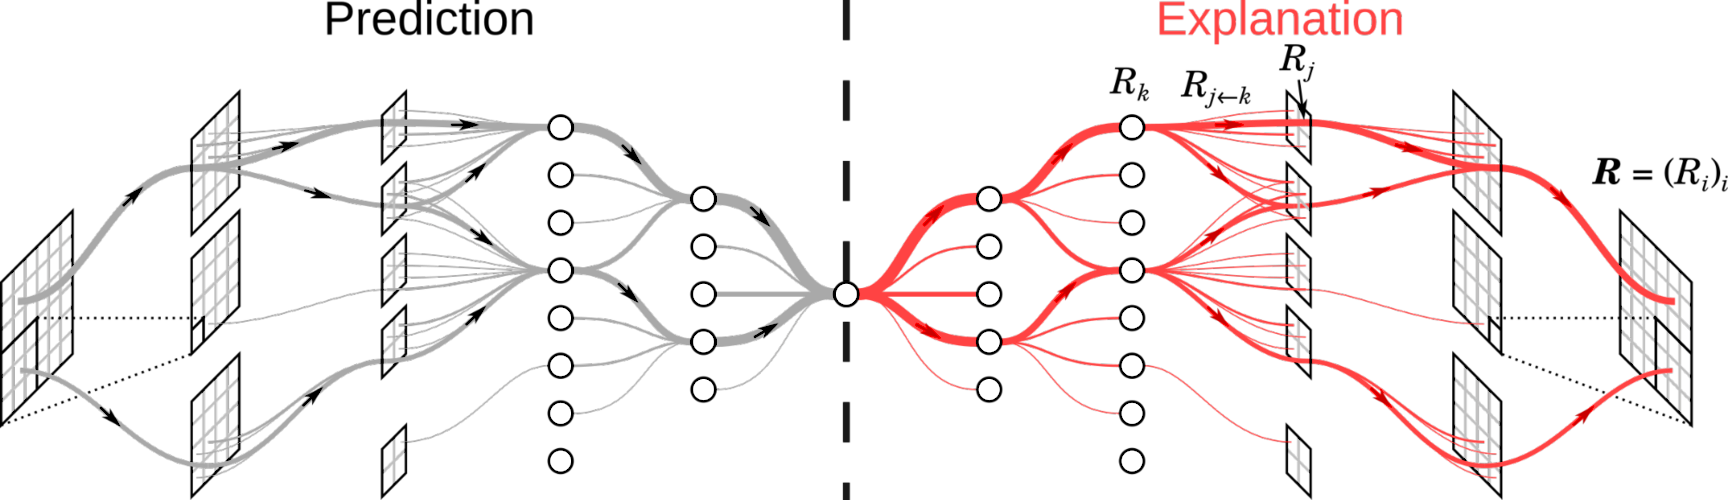
\includegraphics[width=\textwidth]{LRP.png}
    \end{figure}
\end{frame}

\begin{frame}{Layerwise Relevance Propagation}{Propagation rules}
    Initialization:
    \begin{equation}
        R^{(L)}_i = \begin{cases*}
            a^{(L)}_i & if $i = y$\\
            0 & otherwise
        \end{cases*}
    \end{equation}

    LRP-0 rule:
    \begin{equation}
        R^{(l)}_j = \sum_{k}\frac{a^{(l)}_jw_{j, k}}{\sum_{j'}a^{(l)}_{j'}w_{j', k}} R^{(l+1)}_k
    \end{equation}
\end{frame}

\begin{frame}{Layerwise Relevance Propagation}{Results visualization}
    \begin{tabular}[pos]{cc}
        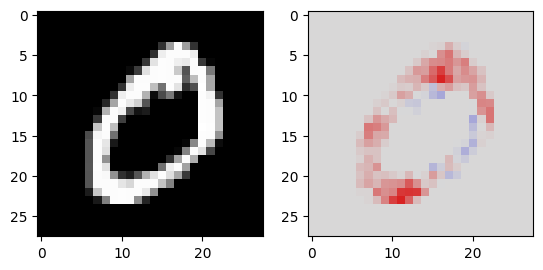
\includegraphics[width=.4\textwidth]{mnist-lrp.png}
        &
        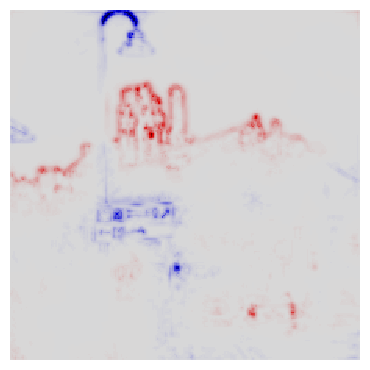
\includegraphics[width=.4\textwidth]{castle-lrp.png}
    \end{tabular}
\end{frame}

\begin{frame}{Pertinence of LRP results}
    \begin{figure}[H]
        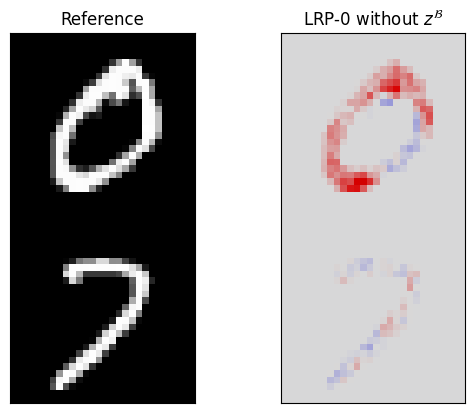
\includegraphics[width=.5\textwidth]{dmnist-lrp.png}
    \end{figure}
\end{frame}

\subsection{Semiring-based provenance annotations}
\begin{frame}{Semiring-based provenance annotations}
    \begin{definition}[Semiring]
        A semiring $(\mathbb{K}, \oplus, \otimes, \mathbf{0}, \mathbf{1})$ is composed of a set $\mathbb{K}$, binary operators $\oplus$ and $\otimes$ such that $\otimes$ distributes over $\oplus$, verifying the following properties:
        \begin{itemize}[label=--, noitemsep]
            \item $(\mathbb{K}, \oplus, \mathbf{0})$ is a commutative monoid
            \item $(\mathbb{K}, \otimes, \mathbf{1})$ is a monoid such that $\mathbf{0}$ is absorbing
        \end{itemize}
    \end{definition}

    \begin{exemple}
        The following structures are semirings:
        \begin{itemize}[label=--, noitemsep]
            \item Real semiring: $(\mathbb{R}, +, \times, 0, 1)$
            \item Boolean semiring: $(\{\bot, \top\}, \lor, \land, \bot, \top)$
            \item Counting semiring: $(\mathbb{N}, +, \times, 0, 1)$
            \item Viterbi semiring: $([0, 1], \max, \times, 0, 1)$
        \end{itemize}
    \end{exemple}
\end{frame}

\section{Extending LRP}

\section{Applications}
\subsection{Image mask computation}
\begin{frame}{Image mask computation}
    
\end{frame}

\subsection{Network pruning using LRP ranking}
\begin{frame}{Network pruning using LRP ranking}
    
\end{frame}

\subsection{Comparison to image perturbation}
\begin{frame}{Comparison to image perturbation}
    \begin{figure}
        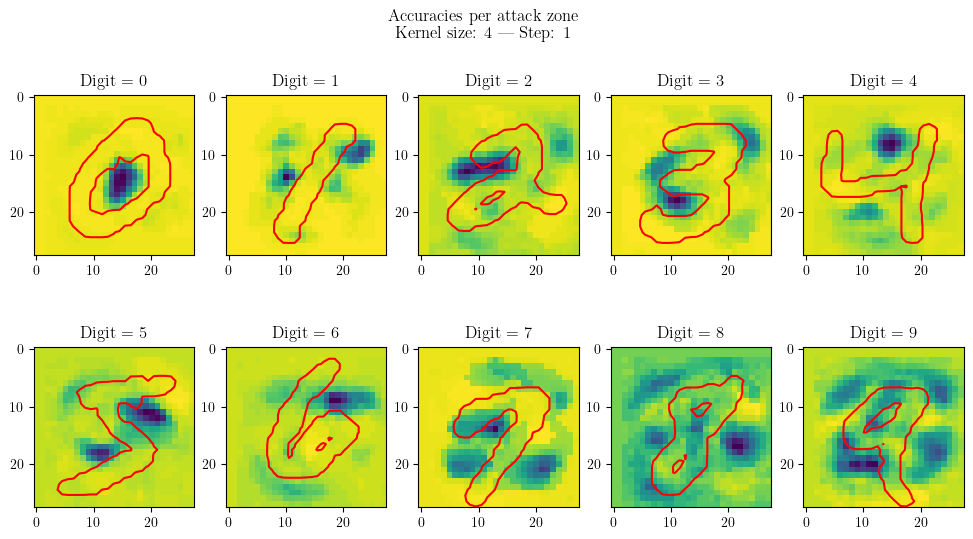
\includegraphics[width=.7\textwidth]{attacks.png}
        \caption{Accuracies per attack zone}
    \end{figure}
\end{frame}

\section{Conclusion}
\begin{frame}
    \nocite{*}
    \printbibliography
\end{frame}

\end{document}